\subsubsection{Module MD-01: Quản lý Lịch làm việc (Scheduling)}

Module Quản lý Lịch làm việc (MD-01) là một thành phần cốt lõi của hệ thống quản lý nhà hàng, được thiết kế để hỗ trợ Quản lý nhà hàng trong việc lập kế hoạch, phân công và theo dõi lịch trình làm việc của nhân viên một cách hiệu quả và tối ưu. Module này bao gồm một loạt các chức năng từ việc định nghĩa các vai trò công việc cơ bản, tạo khung ca làm việc, gán nhân viên cụ thể vào ca, cho đến việc xuất bản lịch và cho phép nhân viên xem lịch trình cá nhân của mình.

\begin{figure}[H]
    \centering
    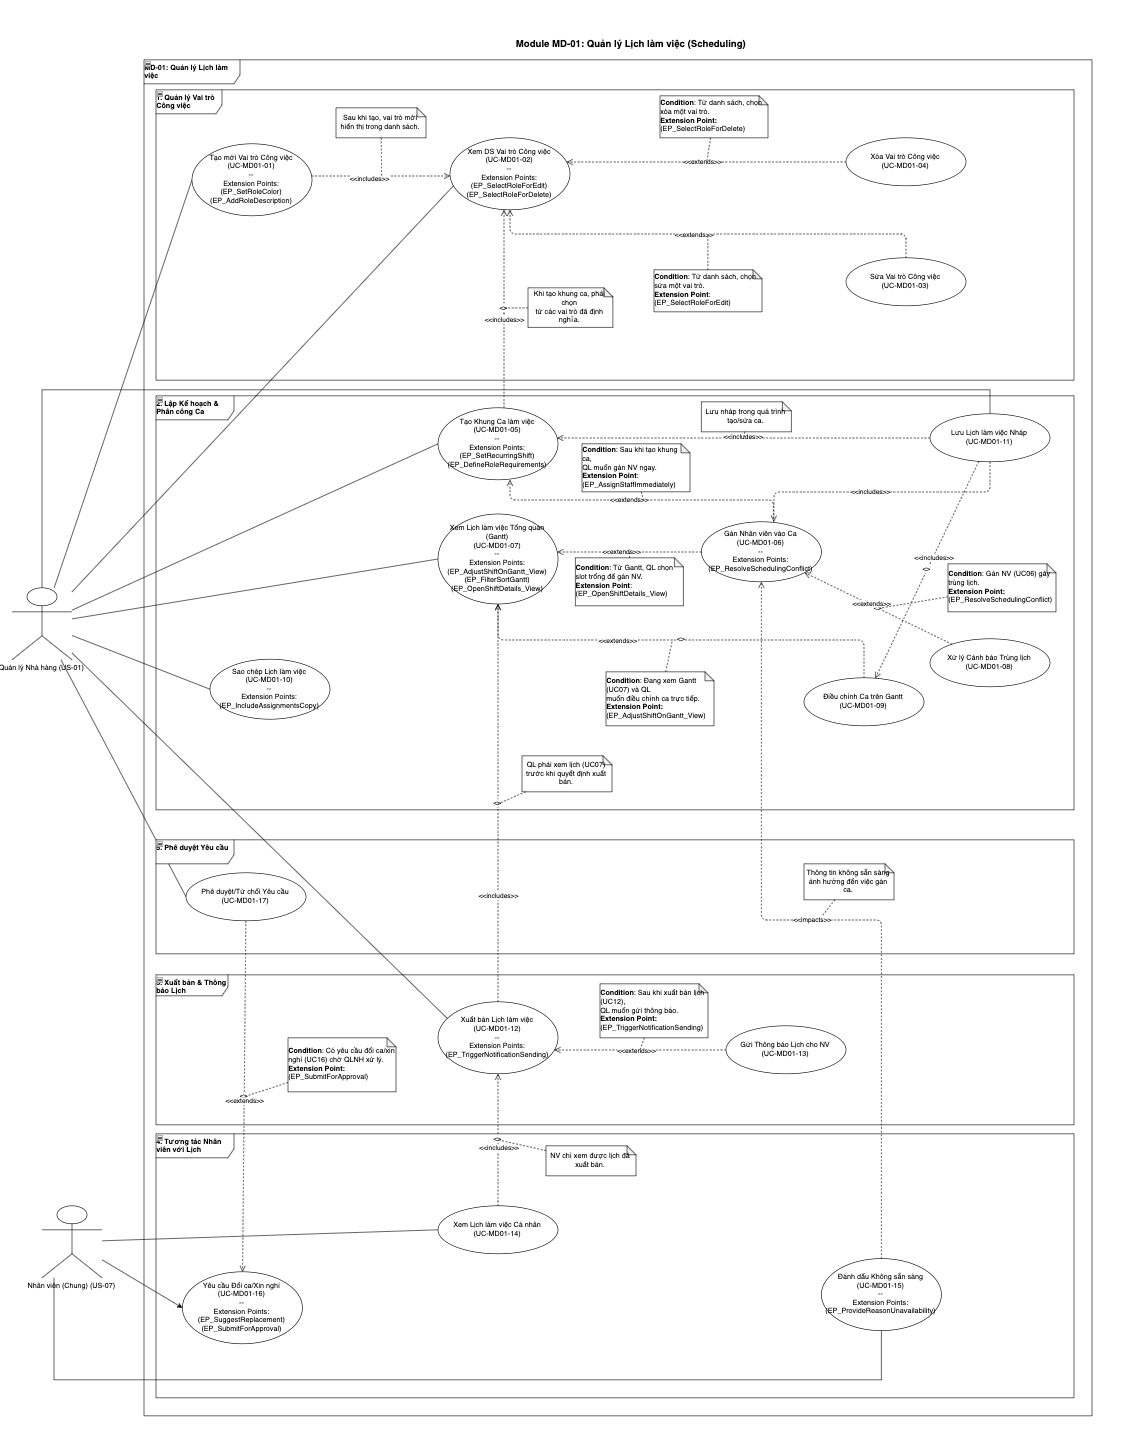
\includegraphics[width=15cm]{Sections/tong_quan/functional_spec/img/uc1.png}
    \vspace{0.5cm}
    \caption{Use case diagram cho Module MD-01}
    \label{fig:my_label}
\end{figure}

\begin{longtable}{|m{2cm}|m{2.5cm}|m{2cm}|m{4cm}|m{4.5cm}|}
    \caption{Danh sách Yêu cầu Chức năng cho Module MD-01: Quản lý Lịch làm việc} \label{tab:fr_md01_revised} \\
    \hline
    \textbf{Mã Module} & \textbf{Mã Yêu cầu CN} & \textbf{Mã Người dùng} & \textbf{Tên Chức năng} & \textbf{Mô tả Ngắn} \\
    \hline
    \endhead
    
    \hline
    \endfoot
    
    \hline
    \endlastfoot
    
    MD-01 & FR-MD01-01 & US-01 & Tạo mới Vai trò Công việc & Cho phép Quản lý nhà hàng định nghĩa một vai trò công việc mới (ví dụ: Bếp trưởng, Phục vụ). \\
    \hline
    MD-01 & FR-MD01-02 & US-01 & Xem Danh sách Vai trò Công việc & Cho phép Quản lý nhà hàng xem danh sách các vai trò công việc đã được định nghĩa. \\
    \hline
    MD-01 & FR-MD01-03 & US-01 & Sửa Thông tin Vai trò Công việc & Cho phép Quản lý nhà hàng chỉnh sửa thông tin của một vai trò công việc hiện có. \\
    \hline
    MD-01 & FR-MD01-04 & US-01 & Xóa Vai trò Công việc & Cho phép Quản lý nhà hàng xóa một vai trò công việc không còn sử dụng (nếu thỏa điều kiện). \\
    \hline
    MD-01 & FR-MD01-05 & US-01 & Tạo Khung Ca làm việc & Cho phép Quản lý nhà hàng định nghĩa các khung ca làm việc (thời gian, ngày, yêu cầu vai trò, số lượng). \\
    \hline
    MD-01 & FR-MD01-06 & US-01 & Gán Nhân viên vào Ca làm việc & Cho phép Quản lý nhà hàng chỉ định nhân viên cụ thể cho các vị trí trong khung ca đã tạo. \\
    \hline
    MD-01 & FR-MD01-07 & US-01 & Xem Lịch làm việc Tổng quan (Gantt) & Hiển thị lịch làm việc của tất cả nhân viên hoặc lọc theo vai trò dưới dạng biểu đồ Gantt. \\
    \hline
    MD-01 & FR-MD01-08 & US-01 & Xử lý Cảnh báo Trùng lịch & Khi hệ thống phát hiện trùng lịch (tự động), cho phép Quản lý nhà hàng xem xét và điều chỉnh việc gán ca để giải quyết xung đột. \\
    \hline
    MD-01 & FR-MD01-09 & US-01 & Điều chỉnh Ca làm việc trên Gantt & Cho phép Quản lý nhà hàng kéo thả, thay đổi kích thước, hoặc sửa đổi trực tiếp các ca trên biểu đồ Gantt. \\
    \hline
    MD-01 & FR-MD01-10 & US-01 & Sao chép Lịch làm việc (Ngày/Tuần/Tùy chỉnh) & Cho phép Quản lý nhà hàng sao chép nhanh lịch của một ngày, một tuần, hoặc một khoảng thời gian tùy chọn sang một thời điểm khác. \\
    \hline
    MD-01 & FR-MD01-11 & US-01 & Lưu Lịch làm việc Nháp & Cho phép Quản lý nhà hàng lưu lại các thay đổi trong lịch trình dưới dạng bản nháp. \\
    \hline
    MD-01 & FR-MD01-12 & US-01 & Xuất bản Lịch làm việc & Cho phép Quản lý nhà hàng công khai (publish) lịch làm việc đã được hoàn thiện. \\
    \hline
    MD-01 & FR-MD01-13 & US-01 & Gửi Thông báo Lịch làm việc cho Nhân viên & Kích hoạt hệ thống gửi thông báo (email/app) đến từng nhân viên về lịch trình cá nhân của họ sau khi lịch được xuất bản. \\
    \hline
    MD-01 & FR-MD01-14 & US-07 & Xem Lịch làm việc Cá nhân & Cho phép Nhân viên xem lịch làm việc đã được xuất bản của riêng mình. \\
    \hline
    MD-01 & FR-MD01-15 & US-07 & Đánh dấu Khoảng thời gian Không sẵn sàng & Cho phép Nhân viên (nếu được cấu hình) thông báo các khoảng thời gian không thể làm việc. \\
    \hline
    MD-01 & FR-MD01-16 & US-07 & Yêu cầu Đổi ca/Xin nghỉ & Cho phép Nhân viên (nếu được cấu hình) gửi yêu cầu đổi ca hoặc xin nghỉ thông qua hệ thống. \\
    \hline
    MD-01 & FR-MD01-17 & US-01 & Phê duyệt/Từ chối Yêu cầu Đổi ca/Xin nghỉ & Cho phép Quản lý nhà hàng xem xét và quyết định các yêu cầu đổi ca/xin nghỉ từ nhân viên. \\
    \hline
    
    \end{longtable}

\subsubsubsection{Mục tiêu và Phạm vi}
\label{sssec:md01_objectives_scope}
Mục tiêu chính của module MD-01 là:
\begin{itemize}
    \item \textbf{Tối ưu hóa việc sử dụng nhân lực:} Đảm bảo đủ nhân sự cho từng ca làm việc dựa trên nhu cầu hoạt động của nhà hàng, tránh tình trạng thiếu hoặc thừa nhân viên.
    \item \textbf{Minh bạch hóa lịch trình:} Cung cấp một cái nhìn tổng quan và chi tiết về lịch làm việc cho cả quản lý và nhân viên, giúp mọi người nắm rõ kế hoạch.
    \item \textbf{Giảm thiểu xung đột lịch trình:} Phát hiện và hỗ trợ giải quyết các trường hợp trùng lịch của nhân viên.
    \item \textbf{Tăng cường hiệu quả quản lý:} Tiết kiệm thời gian và công sức cho Quản lý nhà hàng trong việc lập lịch thủ công.
    \item \textbf{Cải thiện giao tiếp:} Tự động hóa việc thông báo lịch trình mới hoặc thay đổi cho nhân viên.
\end{itemize}
Phạm vi của module bao gồm toàn bộ quy trình quản lý lịch làm việc, từ khâu thiết lập ban đầu (vai trò công việc) đến khi lịch được công bố và nhân viên có thể tương tác (xem lịch, yêu cầu thay đổi).

\subsubsubsection{Đối tượng Sử dụng Chính}
\label{sssec:md01_primary_users}
Module này chủ yếu phục vụ hai nhóm đối tượng người dùng:
\begin{itemize}
    \item \textbf{US-01 (Quản lý nhà hàng):} Là người dùng chính, chịu trách nhiệm thực hiện hầu hết các chức năng của module như tạo vai trò, tạo khung ca, gán nhân viên, điều chỉnh lịch, xuất bản lịch, và phê duyệt các yêu cầu từ nhân viên.
    \item \textbf{US-07 (Nhân viên):} Là người dùng cuối, có thể xem lịch làm việc cá nhân đã được xuất bản, đánh dấu khoảng thời gian không sẵn sàng, và (tùy chọn) gửi yêu cầu đổi ca hoặc xin nghỉ.
\end{itemize}

\subsubsubsection{Các Chức năng Chính}
\label{sssec:md01_key_functionalities}
Module MD-01 cung cấp một bộ các chức năng toàn diện, được mô tả chi tiết qua các Use Case sau:

\begin{itemize}
    \item \textbf{Quản lý Vai trò Công việc (UC-MD01-01 đến UC-MD01-04):}
    \begin{itemize}
        \item Cho phép định nghĩa các vai trò công việc mới (ví dụ: "Đầu bếp chính", "Phục vụ bàn").
        \item Xem danh sách, sửa thông tin, và xóa các vai trò không còn sử dụng (với điều kiện ràng buộc).
    \end{itemize}

    \item \textbf{Lập Kế hoạch và Phân công Ca làm việc (UC-MD01-05, UC-MD01-06, UC-MD01-10, UC-MD01-11):}
    \begin{itemize}
        \item Tạo các khung ca làm việc, xác định thời gian và nhu cầu nhân sự (số lượng, vai trò) cho từng ca.
        \item Gán nhân viên cụ thể vào các vị trí còn trống trong khung ca, dựa trên sự phù hợp về vai trò và tính khả dụng.
        \item Sao chép lịch làm việc từ một ngày/tuần đã có sang ngày/tuần mới để tiết kiệm thời gian.
        \item Lưu trữ các thay đổi dưới dạng lịch nháp trước khi công bố.
    \end{itemize}

    \item \textbf{Trực quan hóa và Điều chỉnh Lịch (UC-MD01-07, UC-MD01-08, UC-MD01-09):}
    \begin{itemize}
        \item Hiển thị lịch làm việc tổng quan dưới dạng biểu đồ Gantt, cho phép lọc và nhóm theo nhân viên hoặc vai trò, thay đổi khung thời gian xem.
        \item Tự động phát hiện và cảnh báo các trường hợp trùng lịch của nhân viên, hỗ trợ Quản lý xử lý.
        \item Cho phép điều chỉnh nhanh ca làm việc (thay đổi thời gian, di chuyển ca, gán lại nhân viên) trực tiếp trên biểu đồ Gantt.
    \end{itemize}

    \item \textbf{Xuất bản và Thông báo Lịch (UC-MD01-12, UC-MD01-13):}
    \begin{itemize}
        \item Chính thức hóa lịch làm việc đã được xếp (chuyển từ "Nháp" sang "Đã xuất bản").
        \item Tự động gửi thông báo lịch làm việc cá nhân đến từng nhân viên sau khi lịch được xuất bản.
    \end{itemize}

    \item \textbf{Tương tác của Nhân viên (UC-MD01-14, UC-MD01-15, UC-MD01-16):}
    \begin{itemize}
        \item Cho phép nhân viên xem lịch làm việc cá nhân đã được xuất bản.
        \item Cho phép nhân viên chủ động đánh dấu các khoảng thời gian họ không thể làm việc.
        \item (Tùy chọn) Cho phép nhân viên gửi yêu cầu đổi ca hoặc xin nghỉ cho các ca đã được phân công.
    \end{itemize}

    \item \textbf{Quản lý Yêu cầu Nhân viên (UC-MD01-17):}
    \begin{itemize}
        \item (Tùy chọn) Cho phép Quản lý nhà hàng xem xét và phê duyệt hoặc từ chối các yêu cầu đổi ca/xin nghỉ từ nhân viên.
    \end{itemize}
\end{itemize}

\subsubsubsection{Tóm tắt Luồng Hoạt động Tổng thể}
\label{sssec:md01_overall_workflow}
Luồng hoạt động chính trong module MD-01 thường diễn ra như sau:
\begin{enumerate}
    \item \textbf{Thiết lập ban đầu:} Quản lý nhà hàng định nghĩa các Vai trò Công việc cần thiết (UC-MD01-01).
    \item \textbf{Tạo khung ca:} Quản lý tạo các Khung Ca làm việc cho một khoảng thời gian (ví dụ: tuần), xác định nhu cầu về số lượng và vai trò cho mỗi ca (UC-MD01-05). Có thể sử dụng chức năng Sao chép lịch để tăng tốc (UC-MD01-10).
    \item \textbf{Phân công nhân viên:} Quản lý gán từng Nhân viên cụ thể vào các vị trí trong khung ca (UC-MD01-06). Hệ thống hỗ trợ bằng cách gợi ý nhân viên phù hợp và cảnh báo nếu có thông tin không sẵn sàng (UC-MD01-15).
    \item \textbf{Rà soát và điều chỉnh:} Quản lý xem Lịch làm việc Tổng quan trên Gantt (UC-MD01-07), phát hiện và Xử lý Cảnh báo Trùng lịch (UC-MD01-08), và thực hiện các Điều chỉnh Ca cần thiết (UC-MD01-09). Mọi thay đổi được Lưu Nháp (UC-MD01-11).
    \item \textbf{Xuất bản và thông báo:} Sau khi hoàn tất, Quản lý Xuất bản Lịch làm việc (UC-MD01-12), và hệ thống Gửi Thông báo cho Nhân viên (UC-MD01-13).
    \item \textbf{Nhân viên tương tác:} Nhân viên Xem Lịch làm việc Cá nhân (UC-MD01-14). Nếu được phép, họ có thể Yêu cầu Đổi ca/Xin nghỉ (UC-MD01-16).
    \item \textbf{Xử lý yêu cầu:} Quản lý Phê duyệt/Từ chối các yêu cầu từ nhân viên (UC-MD01-17), và cập nhật lại lịch nếu cần.
\end{enumerate}
Module MD-01 đóng vai trò trung tâm trong việc đảm bảo hoạt động trơn tru hàng ngày của nhà hàng bằng cách quản lý hiệu quả nguồn lực quan trọng nhất: con người.
